\chapter{Vzorový IDEA záznam}
\label{code:idea}

\begin{figure}[ht]
\lstset{basicstyle=\small,style=JSON}
\begin{lstlisting}
{
    "Format" :      "IDEA0",
    "ID" :          "73e0b136-aeb8-4aae-bb80-9bfb4f258847",
    "Category" :    ["Availibility.DDoS"],
    "Description" : "DNS amplification",
    "EventTime" :   "2016-04-07T22:19:25Z",
    "CreateTime" :  "2016-04-07T22:34:52Z",
    "CeaseTime" :   "2016-04-07T22:34:38Z",
    "DetectTime" :  "2016-04-07T22:34:38Z"
    "PacketCount" : 393,
    "Source" : [{
        "IP4" : ["192.1.0.201"],
        "Proto" : ["udp","dns"],
        "OutPacketCount" : 393,
        "InPacketCount" : 767
    }],
    "Target" : [{
        "Proto" : ["udp","dns"],
        "IP4" : ["10.0.0.135"],
        "InPacketCount" : 393
    }],
    "Node" : [{
        "SW" : ["NEMEA","amplification_detection"],
        "Name" : "cz.cesnet.nemea.amplification_detection"
    }],
    "Type" : ["Flow","Statistical"],
}
\end{lstlisting}
\captionof{lstlisting}{Vzorový IDEA záznam ze systému NEMEA. Některé části byly vynechány nebo zkráceny a IP adresy anonymizovány.}
\end{figure}


\chapter{Drátěné modely aplikace}

\begin{figure}[ht]
    \centering
    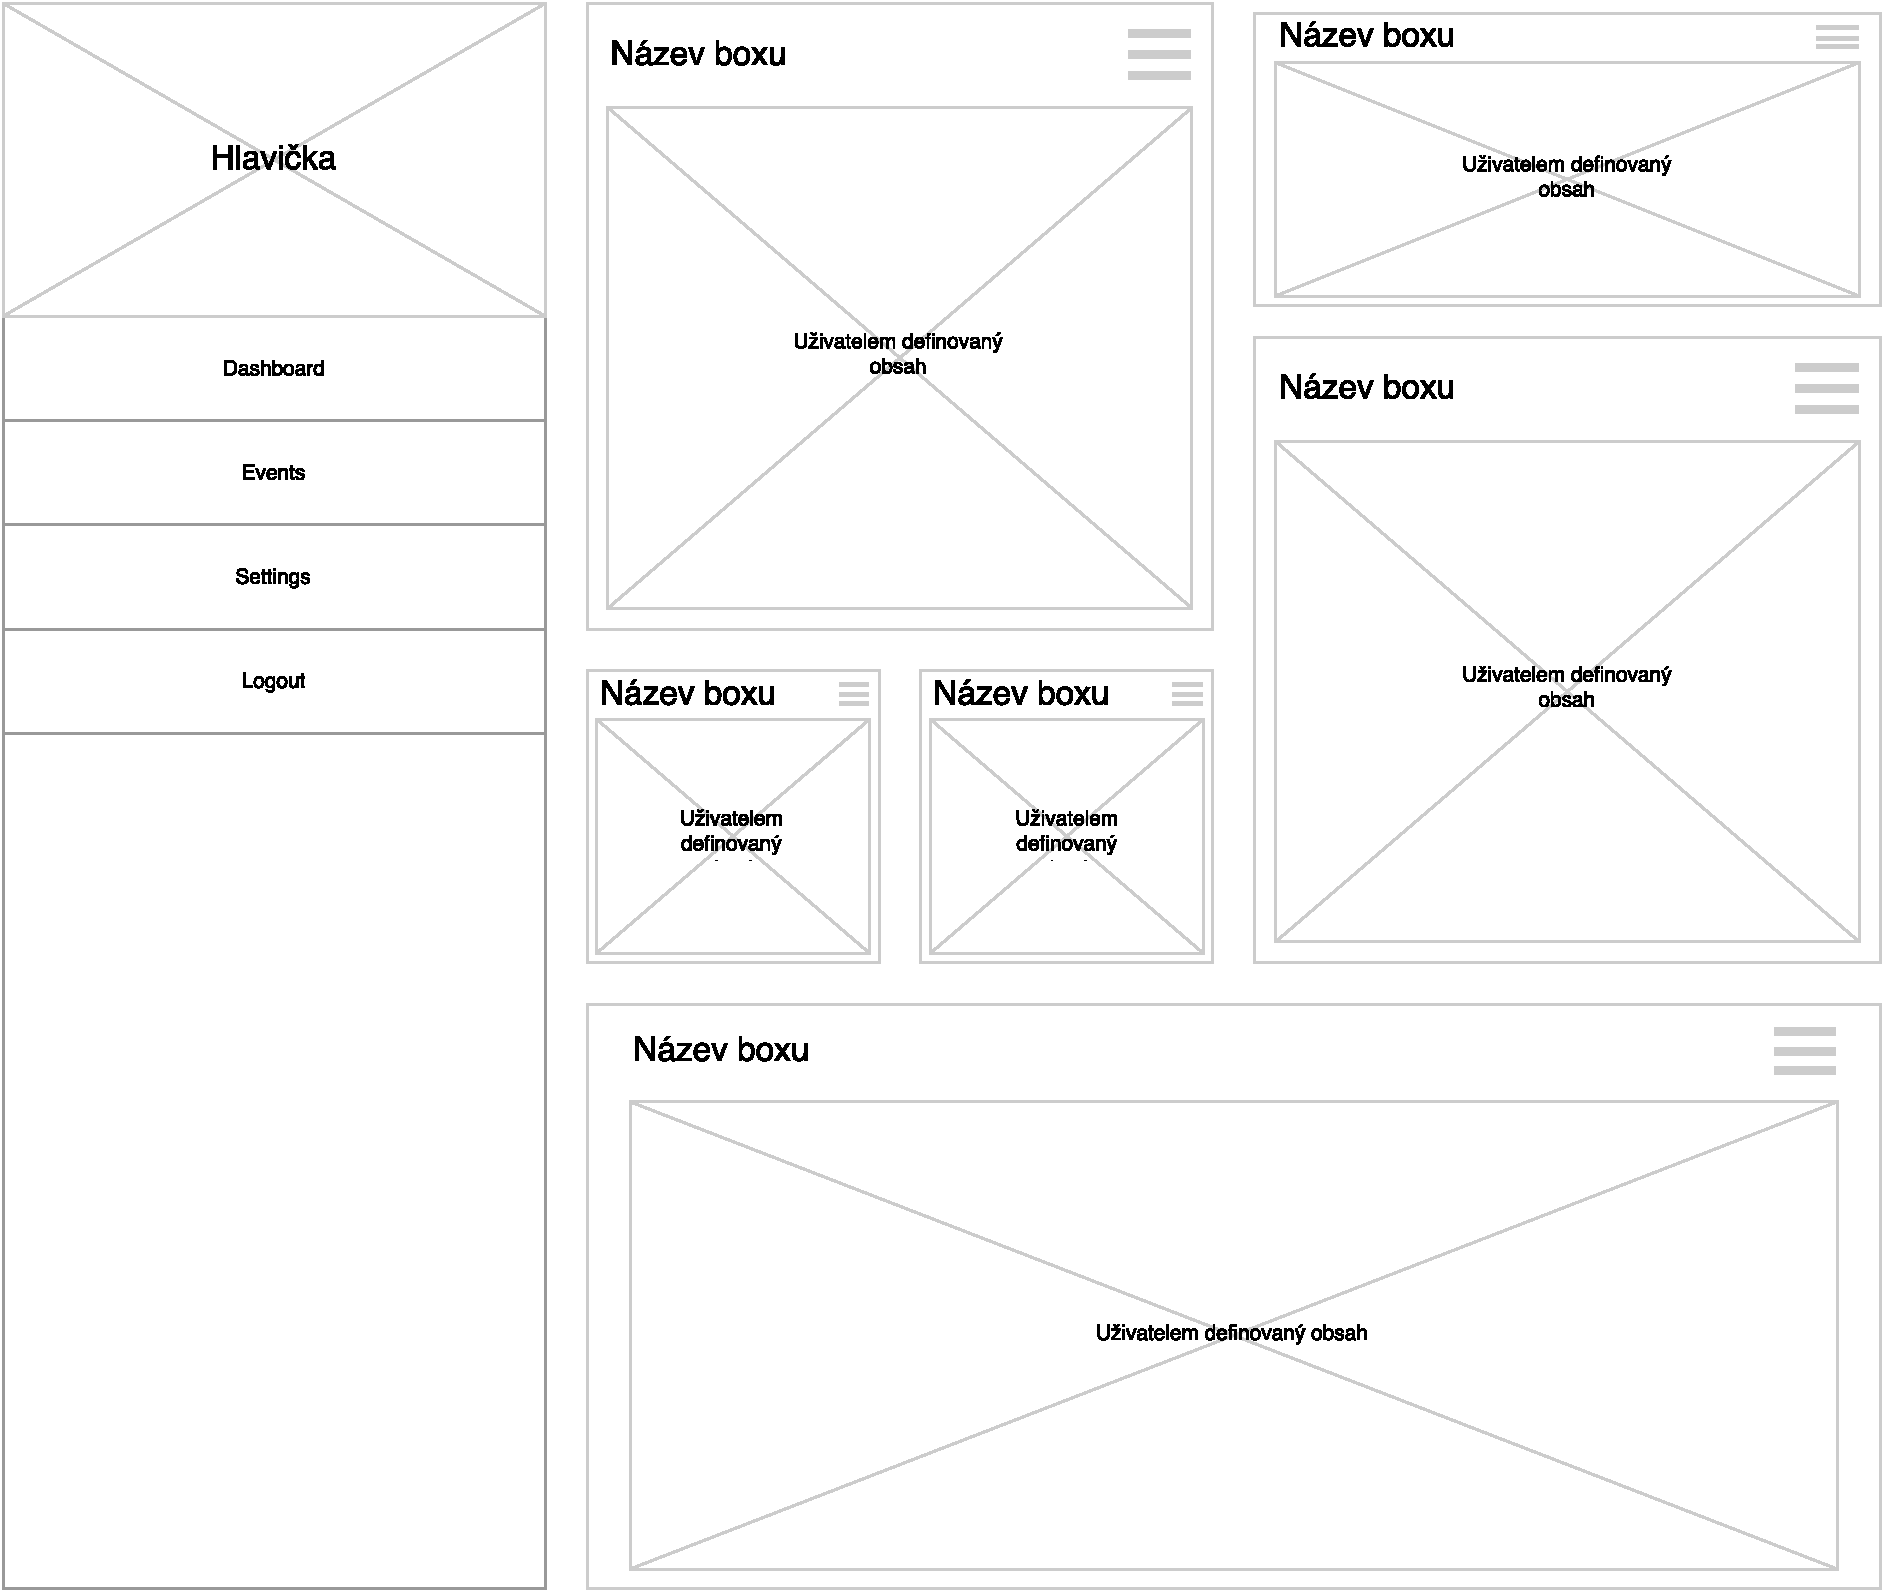
\includegraphics[width=1\textwidth]{fig/wf_dashboard.pdf}
    \caption{Drátěný model pro dashboard, který uživatel může konfigurovat.} \label{wf:dashboard}
\end{figure}

\begin{figure}[ht]
    \centering
    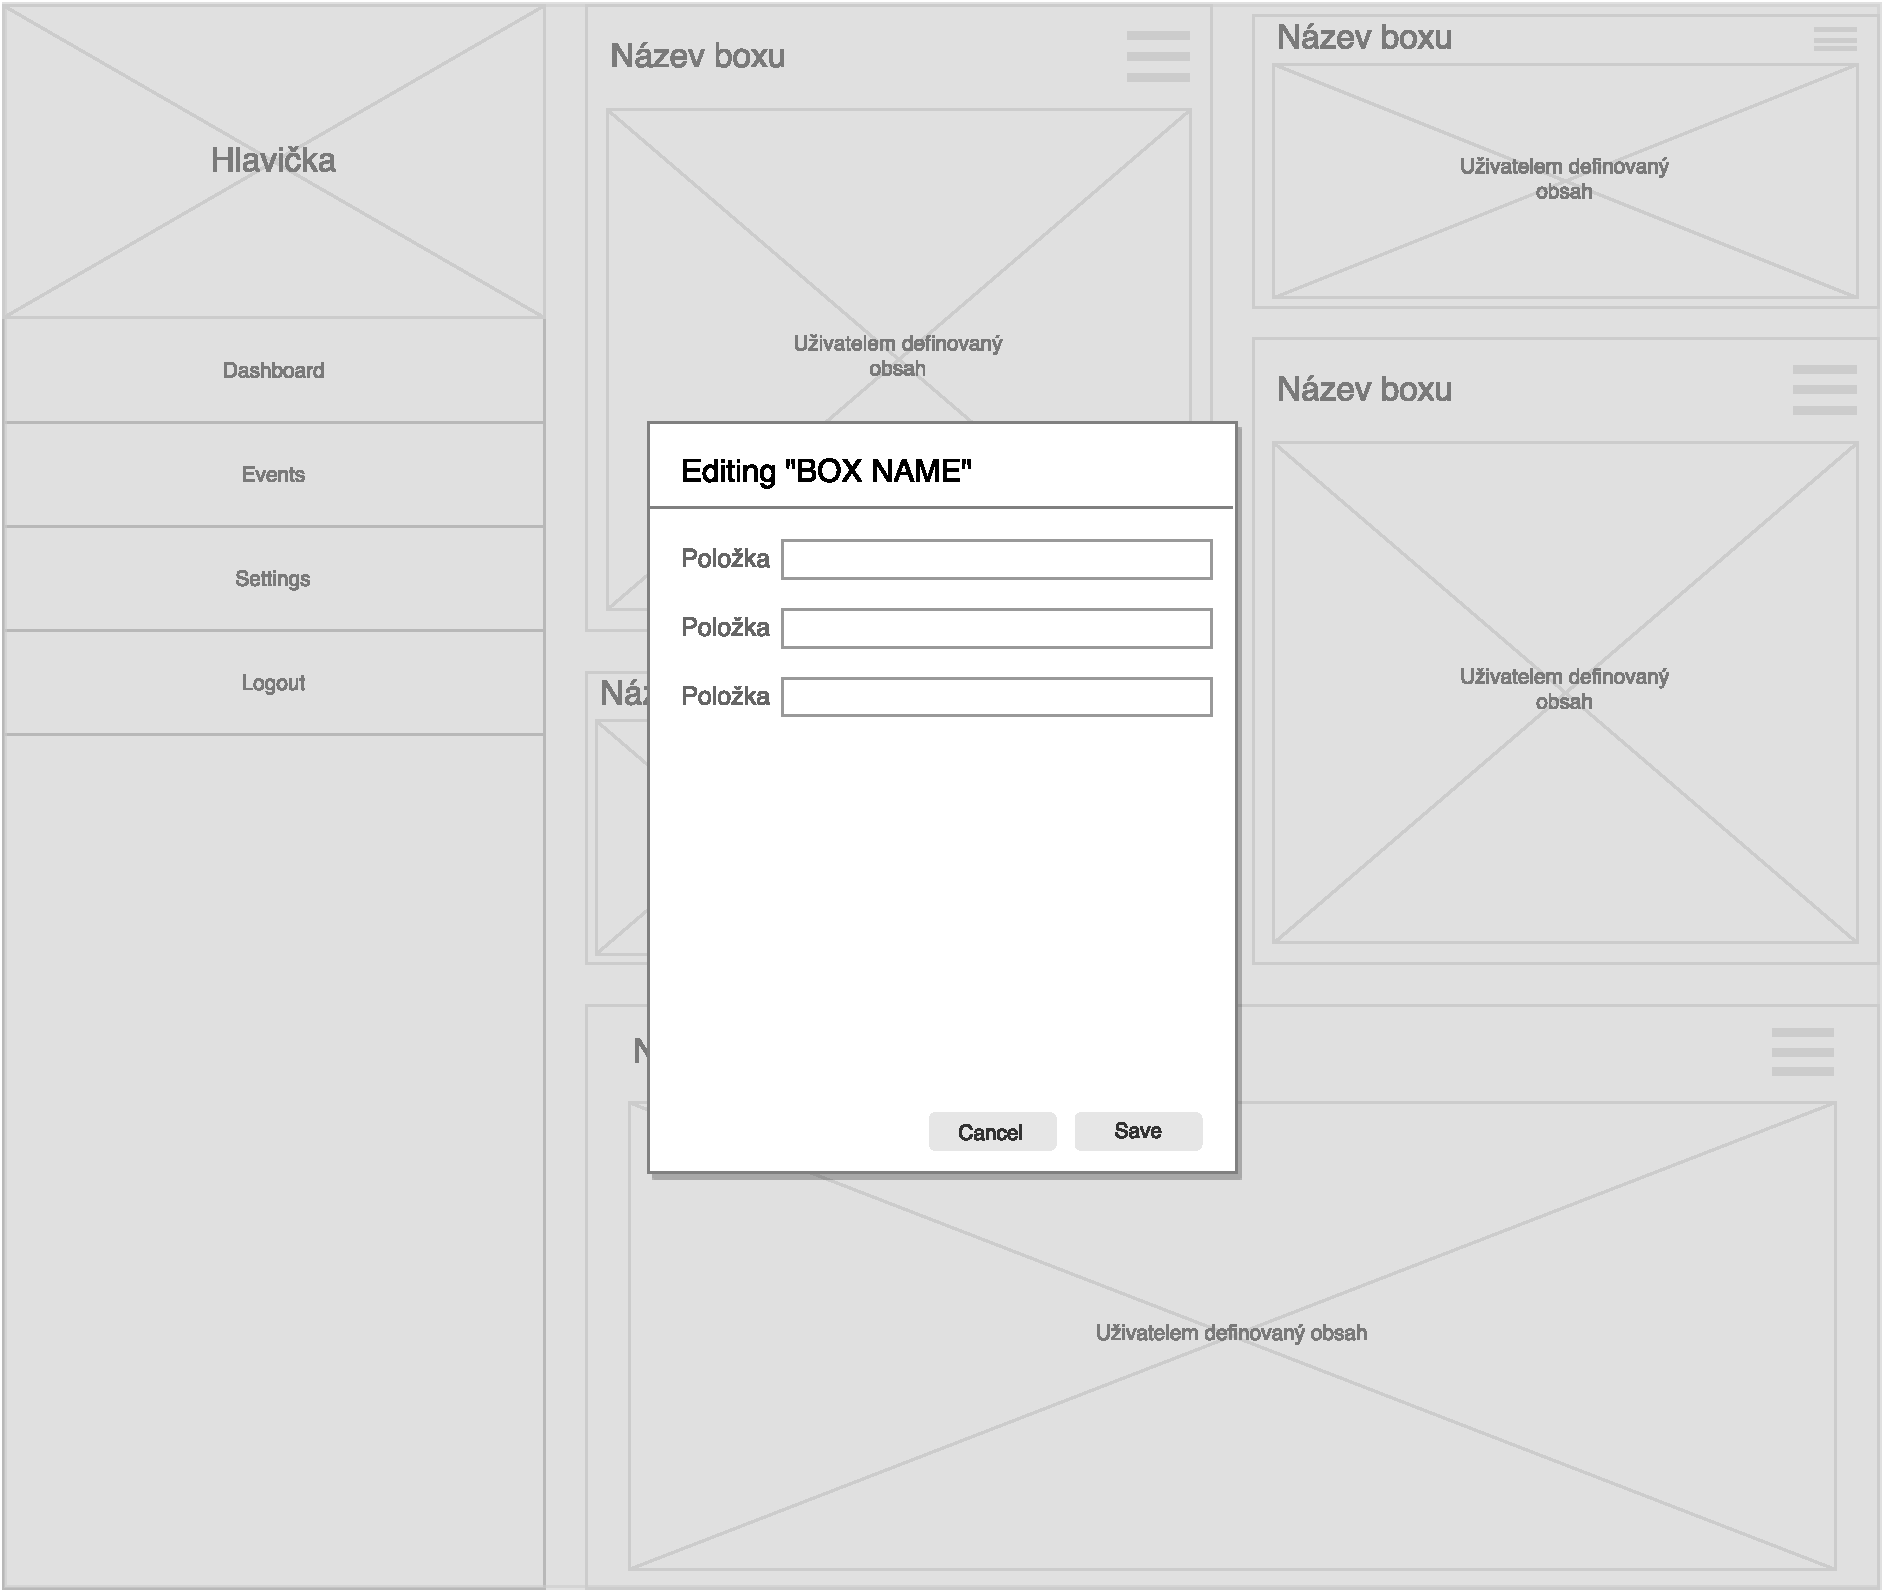
\includegraphics[width=1\textwidth]{fig/wf_dashboard_edit.pdf}
    \caption{Konfigurace boxu v dashboardu.} \label{wf:dashboard_edit}
\end{figure}


\begin{figure}[ht]
    \centering
    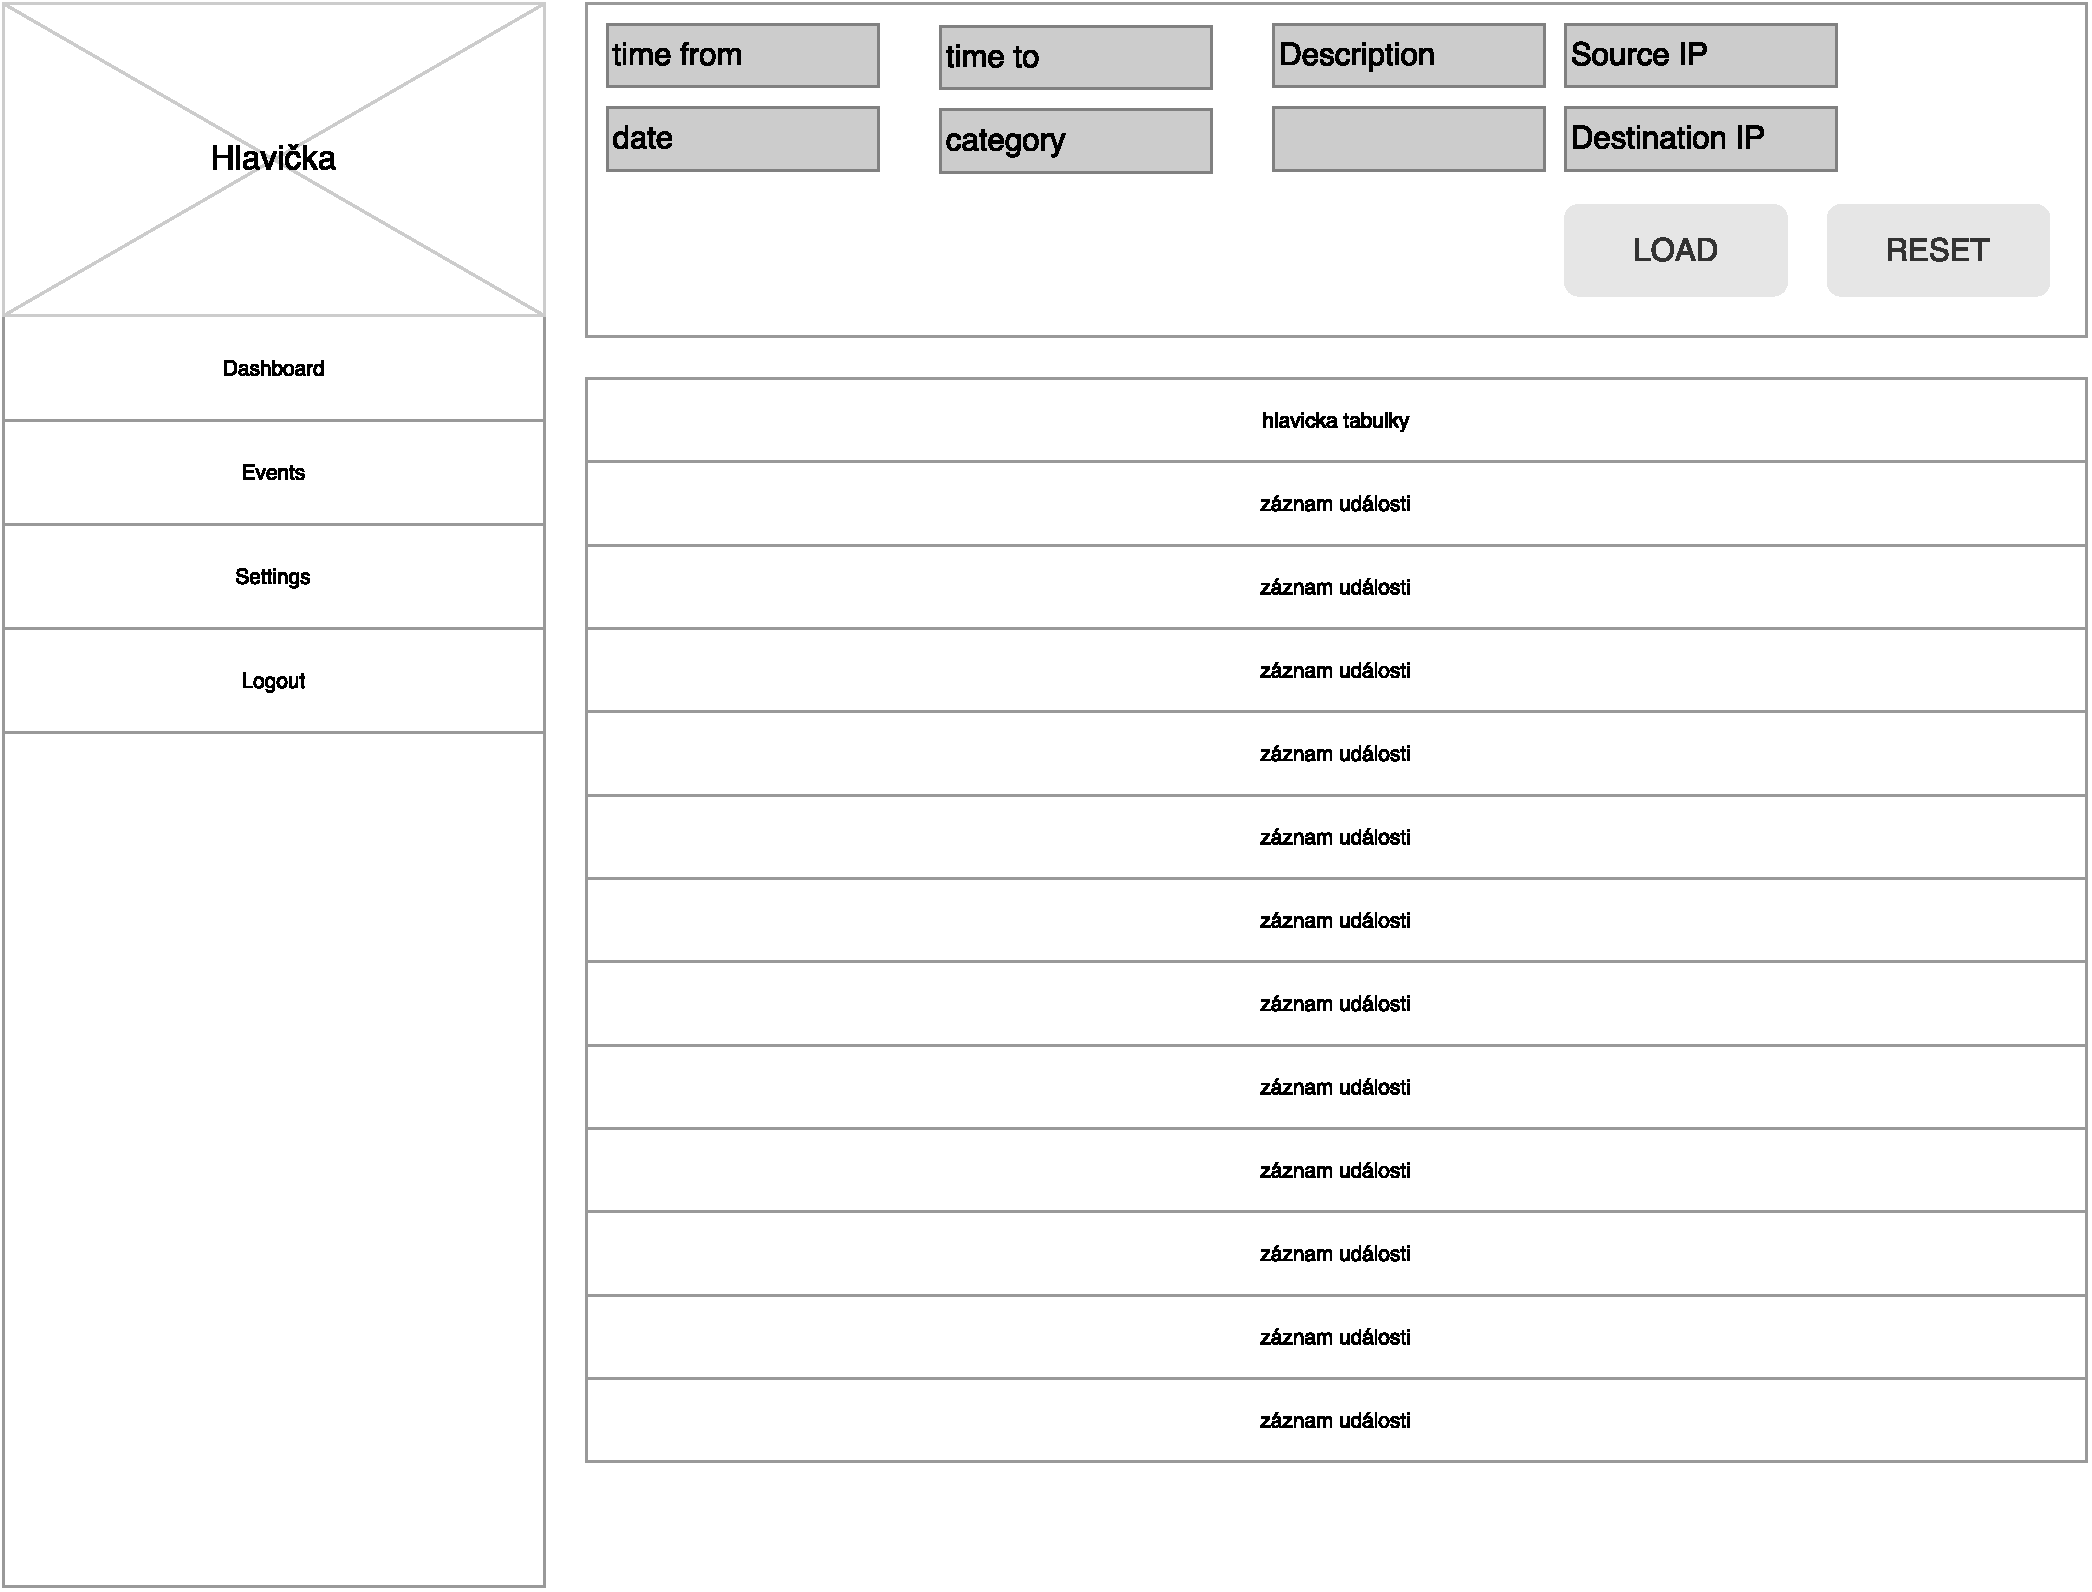
\includegraphics[width=1\textwidth]{fig/wf_dashboard_events.pdf}
    \caption{Přehled vyfiltrovaných událostí.} \label{wf:dashboard_events}
\end{figure}

\chapter{Seznam použitých Python knihoven}

\begin{figure}[ht]
\lstset{basicstyle=\small,style=JSON}
\begin{lstlisting}
Flask==0.10.1
Flask-Cors==2.1.2
itsdangerous==0.24
Jinja2==2.8
MarkupSafe==0.23
py-bcrypt==0.4
pycparser==2.14
PyJWT==1.4.0
pymongo==3.2
six==1.10.0
Werkzeug==0.11.3
\end{lstlisting}
\captionof{lstlisting}{Obsah souboru requirements.txt, který využívá nástroj pip pro instalaci Python knihoven.}
\label{code:requirements}
\end{figure}

\chapter{Snímky uživatelské strany před akceptačními testy}
\label{screens:before}

\begin{figure}[ht]
    \centering
    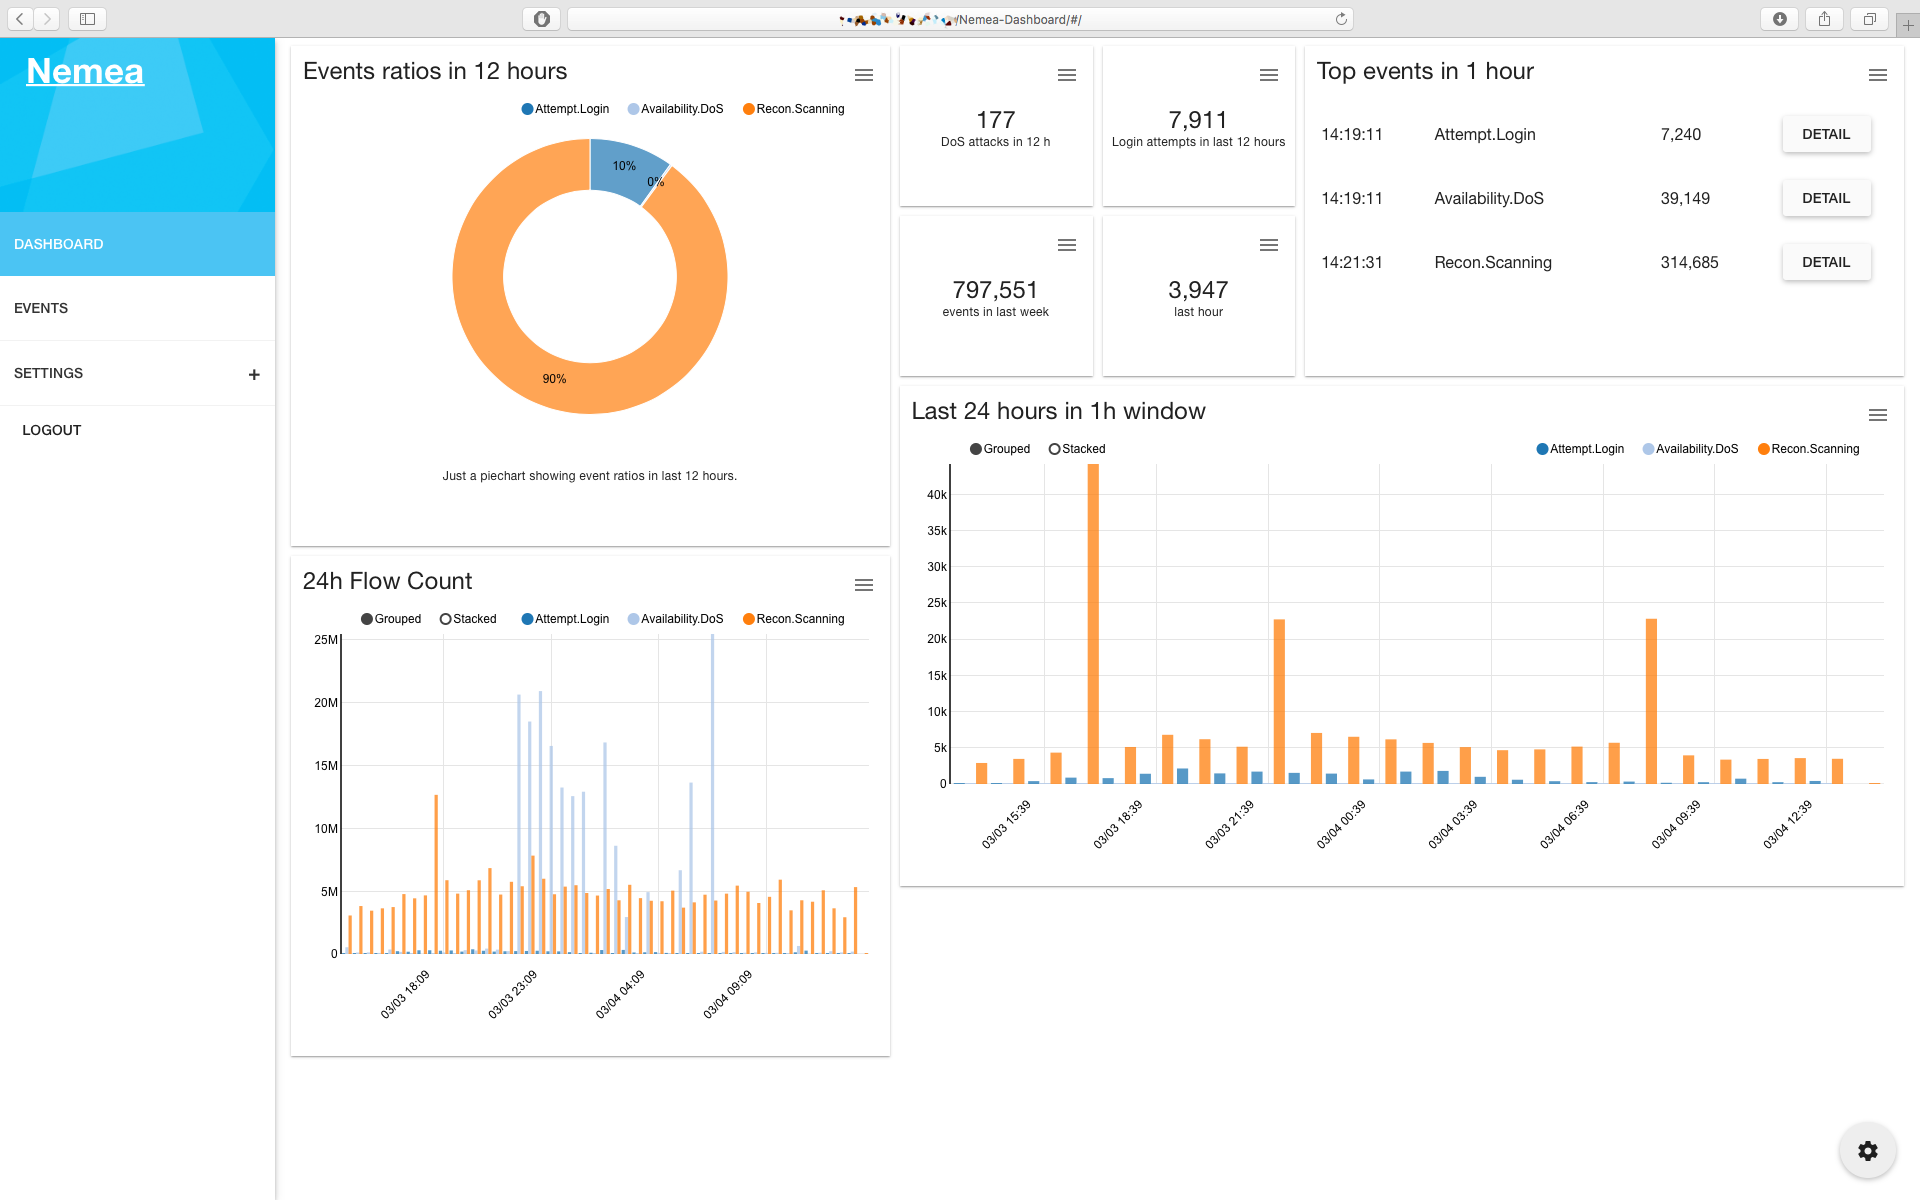
\includegraphics[width=1\textwidth]{fig/screen_before_1.png}
    \caption{Úvodní obrazovka s přednastavenými boxy.} \label{screen:before:1}
\end{figure}

\begin{figure}[ht]
    \centering
    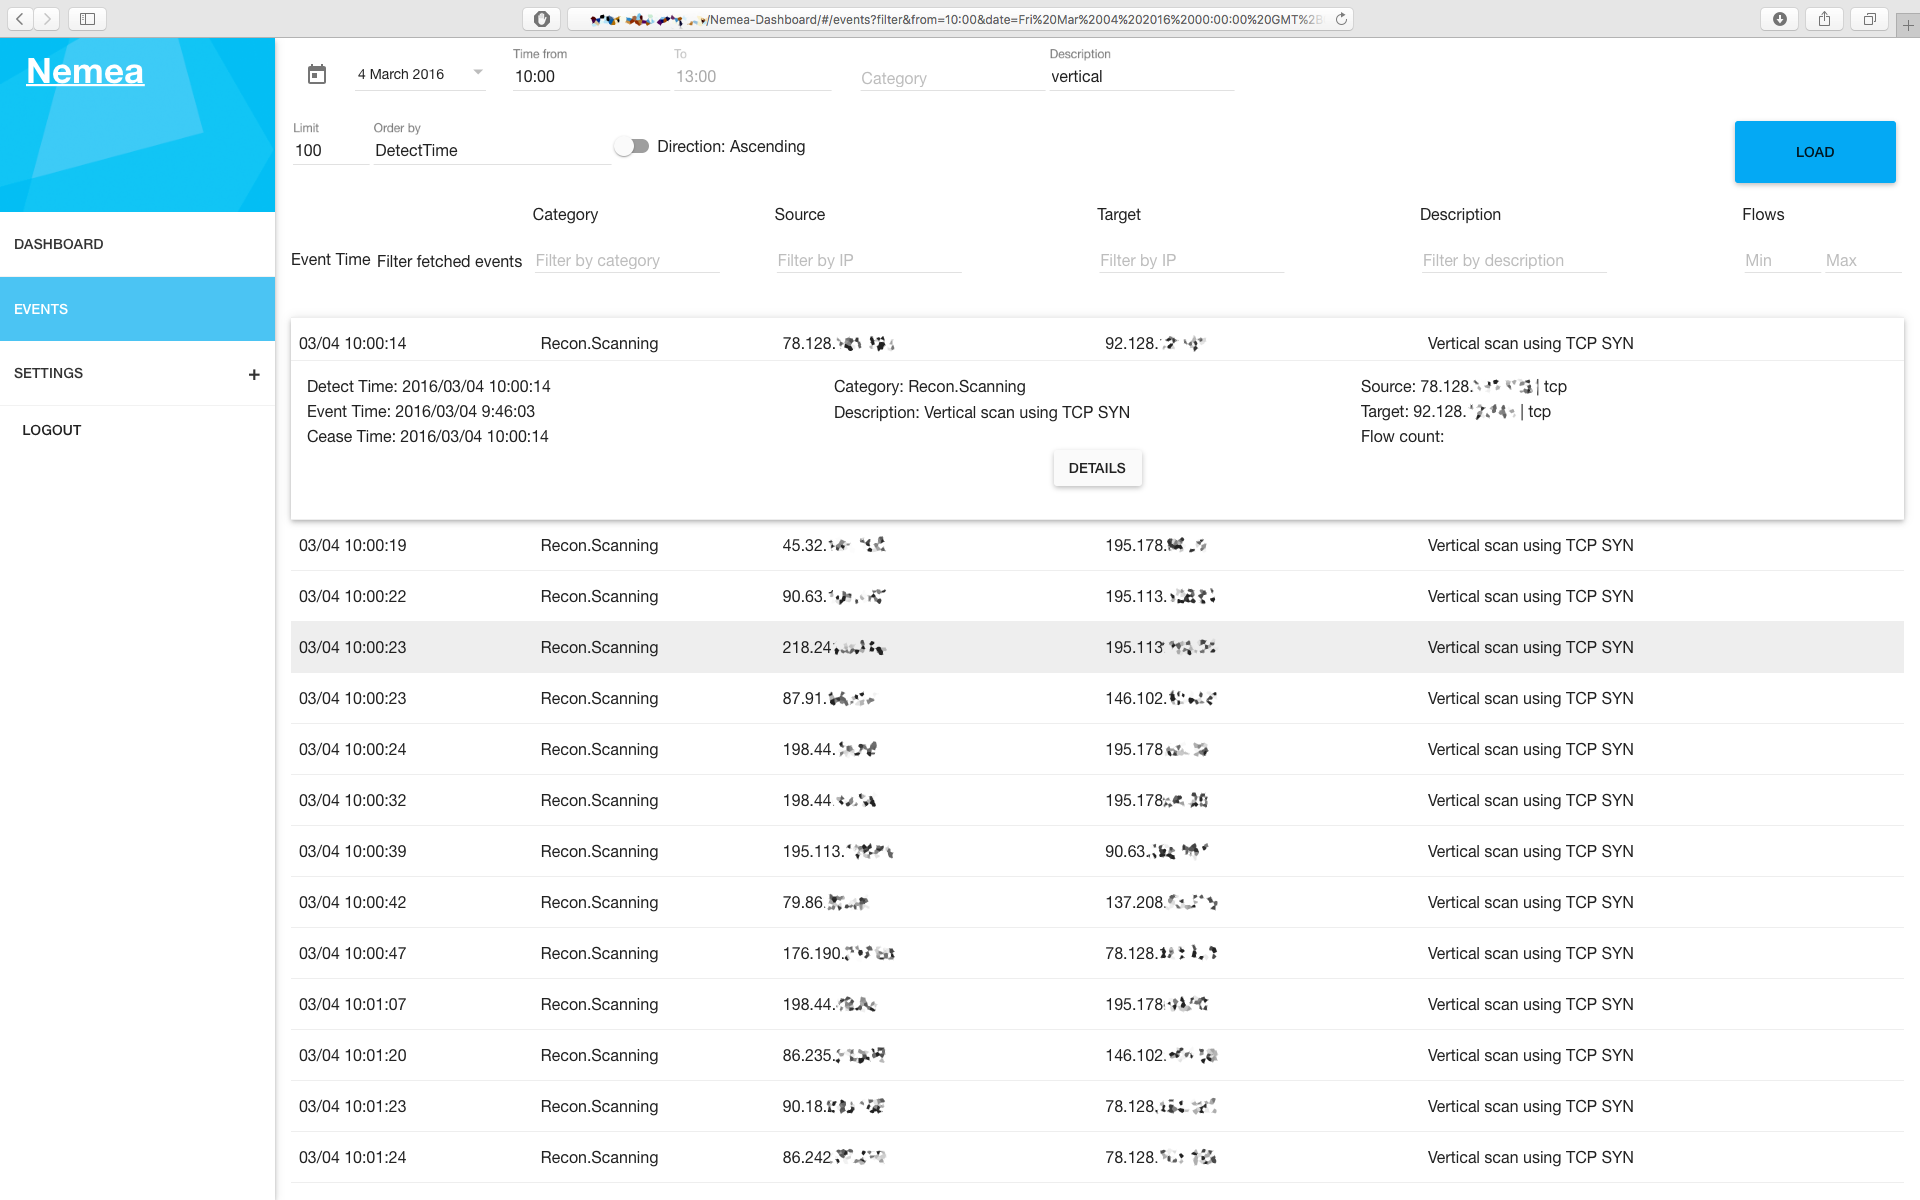
\includegraphics[width=1\textwidth]{fig/screen_before_2.png}
    \caption{Výpis nalezených událostí.} \label{screen:before:2}
\end{figure}

\begin{figure}[ht]
    \centering
    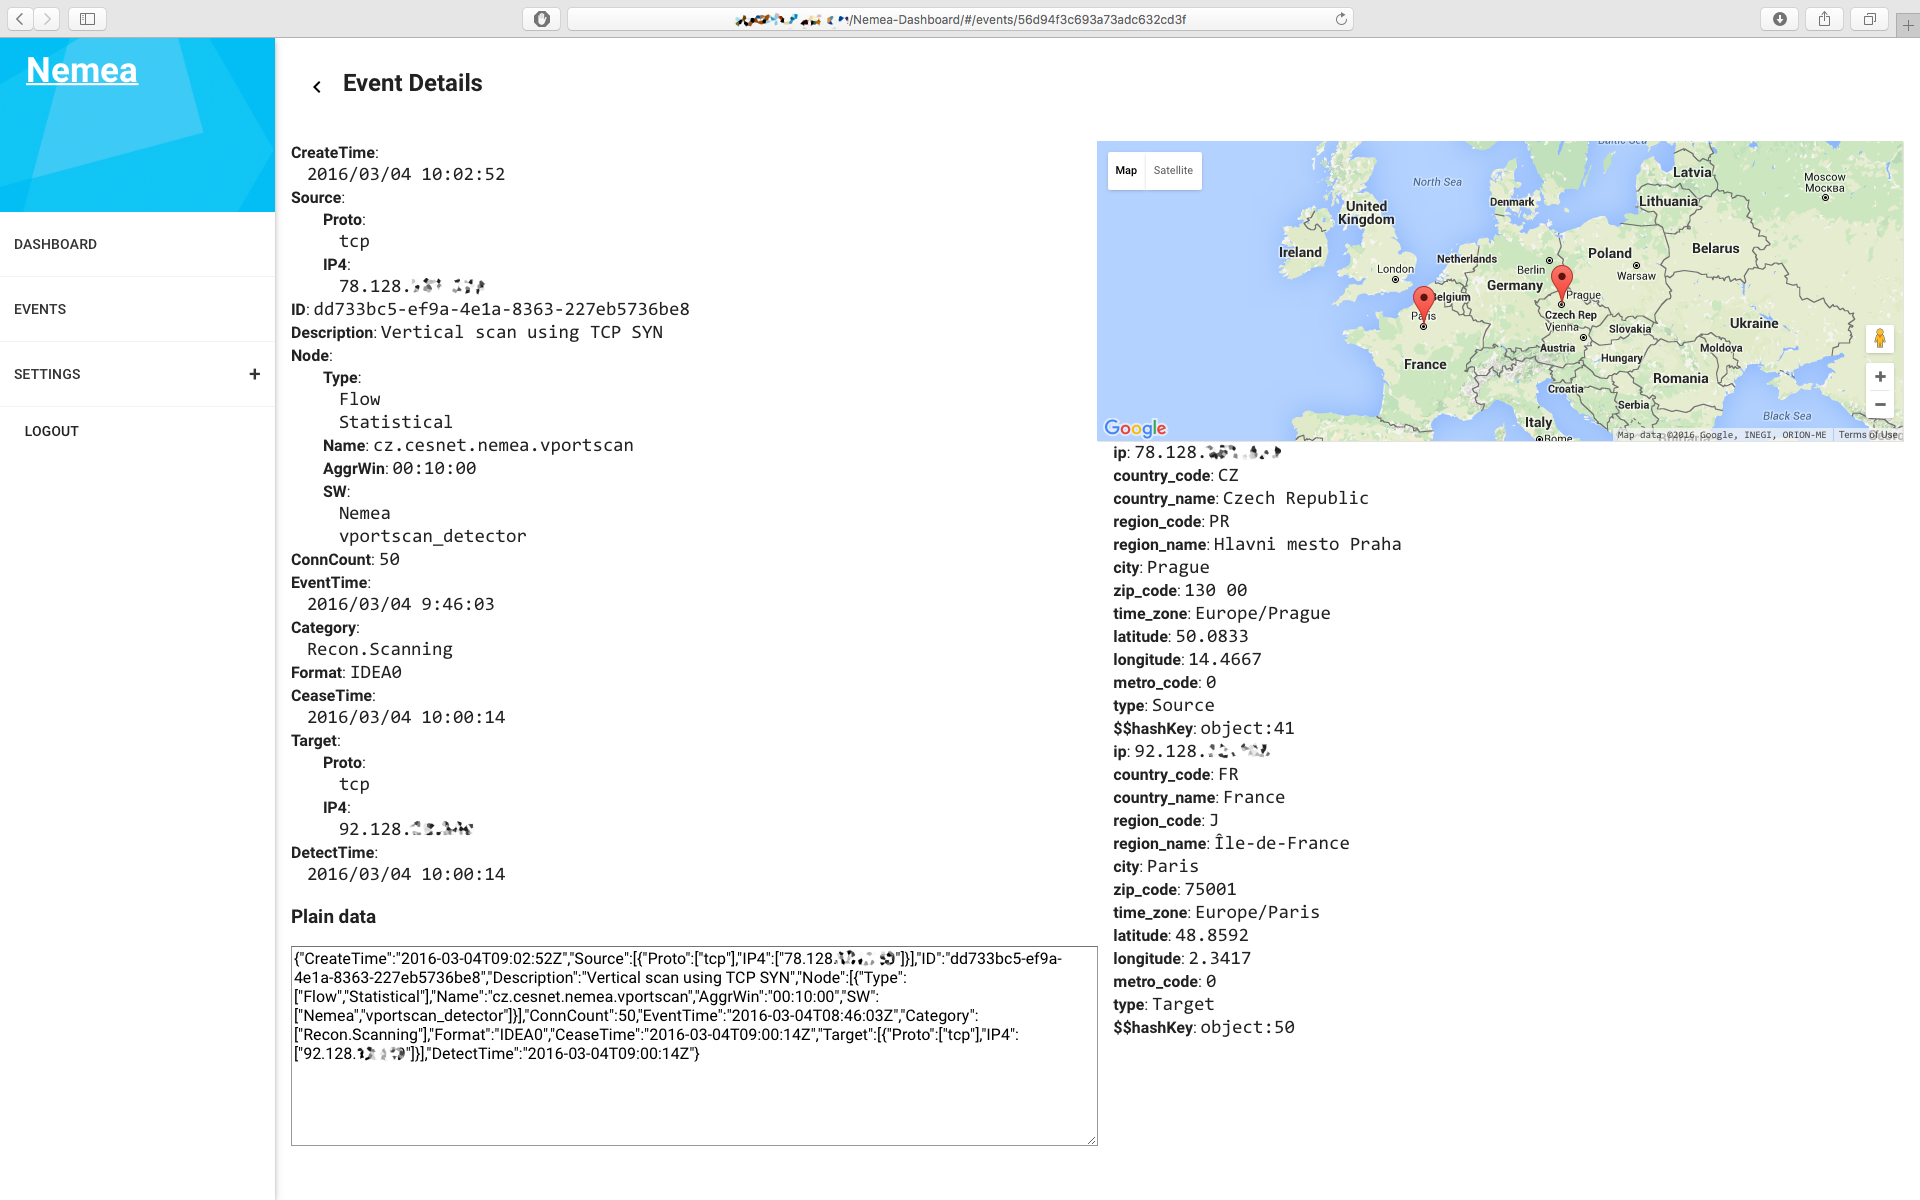
\includegraphics[width=1\textwidth]{fig/screen_before_3.png}
    \caption{Detail události.} \label{screen:before:3}
\end{figure}



\chapter{Snímky uživatelské strany po prvním kole testů}
\label{screens:after}

\begin{figure}[ht]
    \centering
    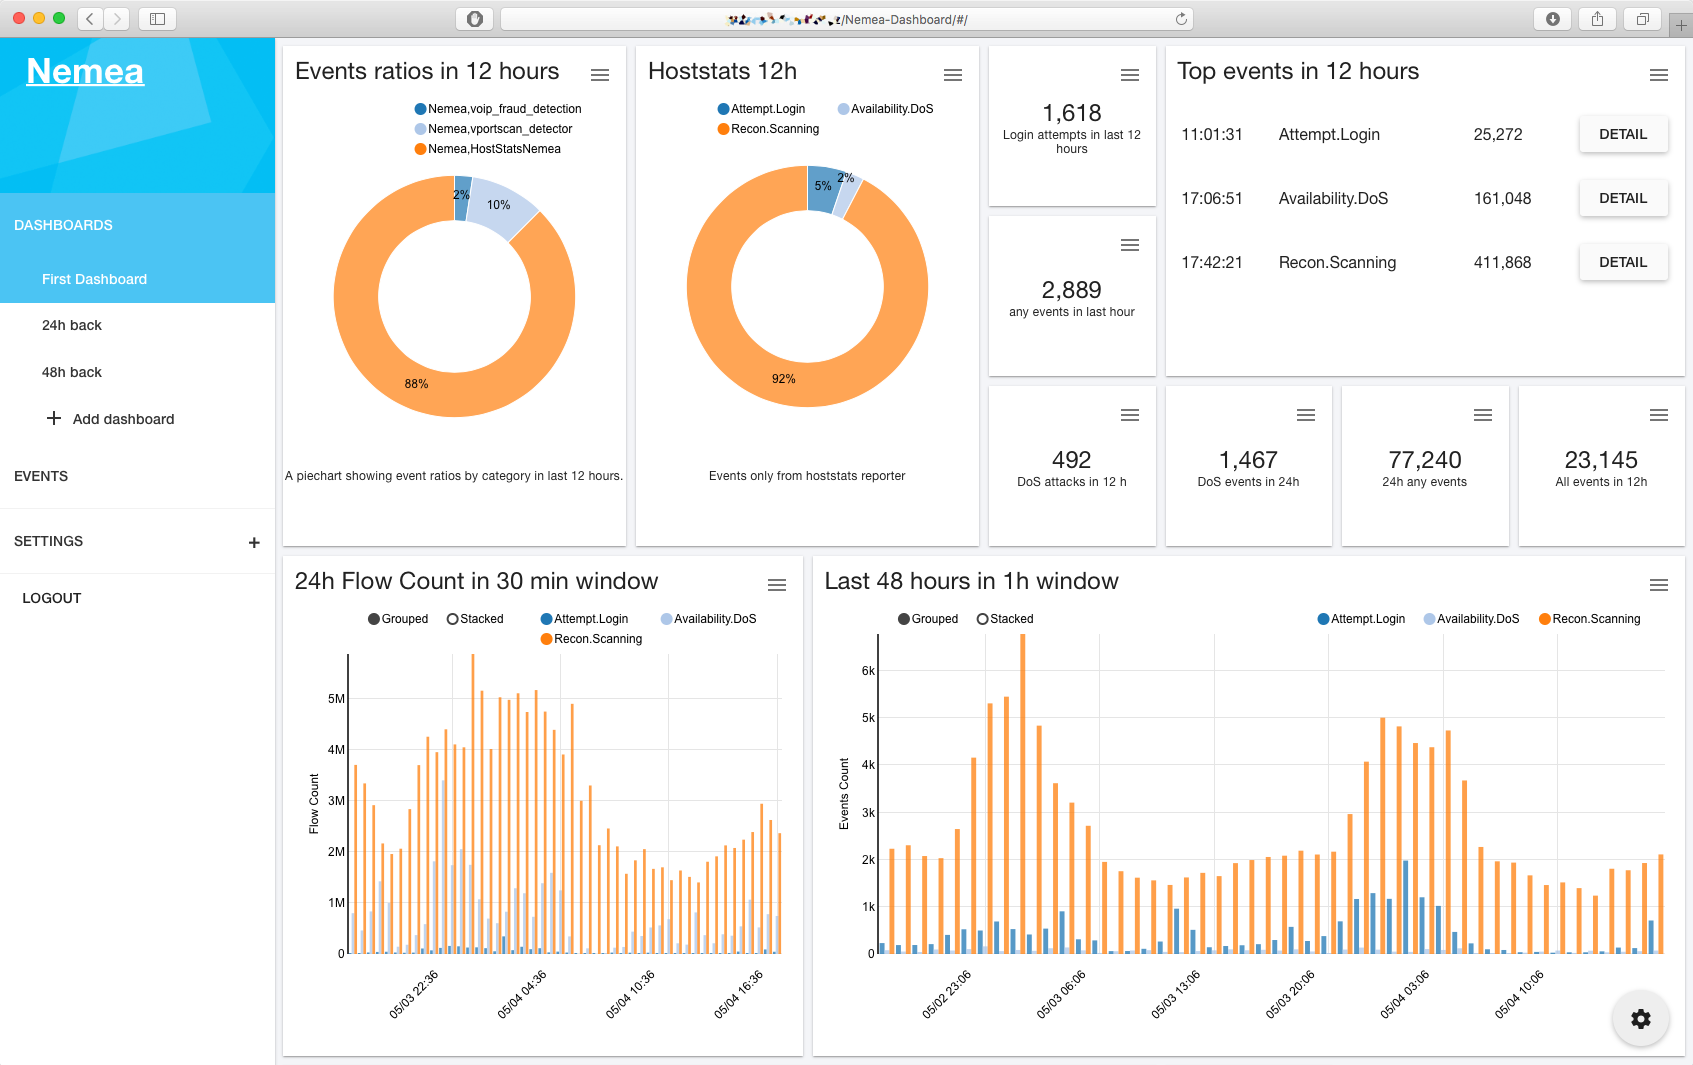
\includegraphics[width=1\textwidth]{fig/screen_after_1.png}
    \caption{Úvodní obrazovka s přednastavenými boxy.} \label{screen:after:1}
\end{figure}

\begin{figure}[ht]
    \centering
    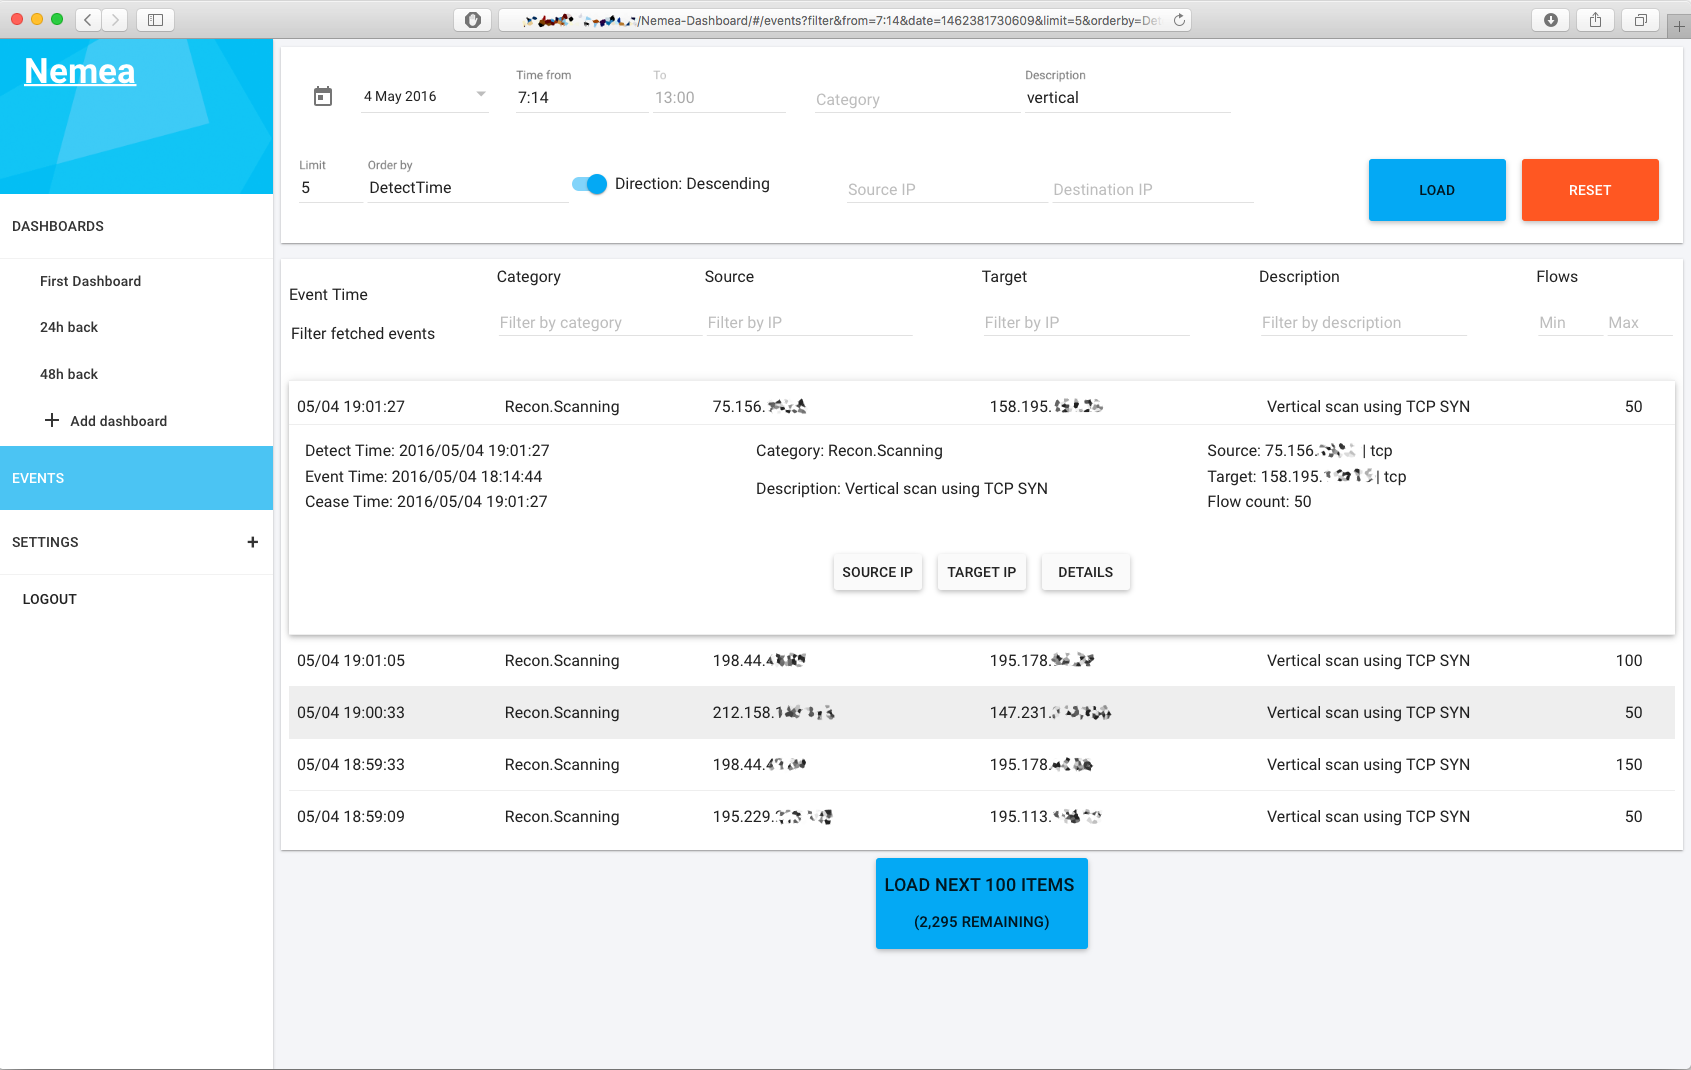
\includegraphics[width=1\textwidth]{fig/screen_after_2.png}
    \caption{Výpis nalezených událostí.} \label{screen:after:2}
\end{figure}

\begin{figure}[ht]
    \centering
    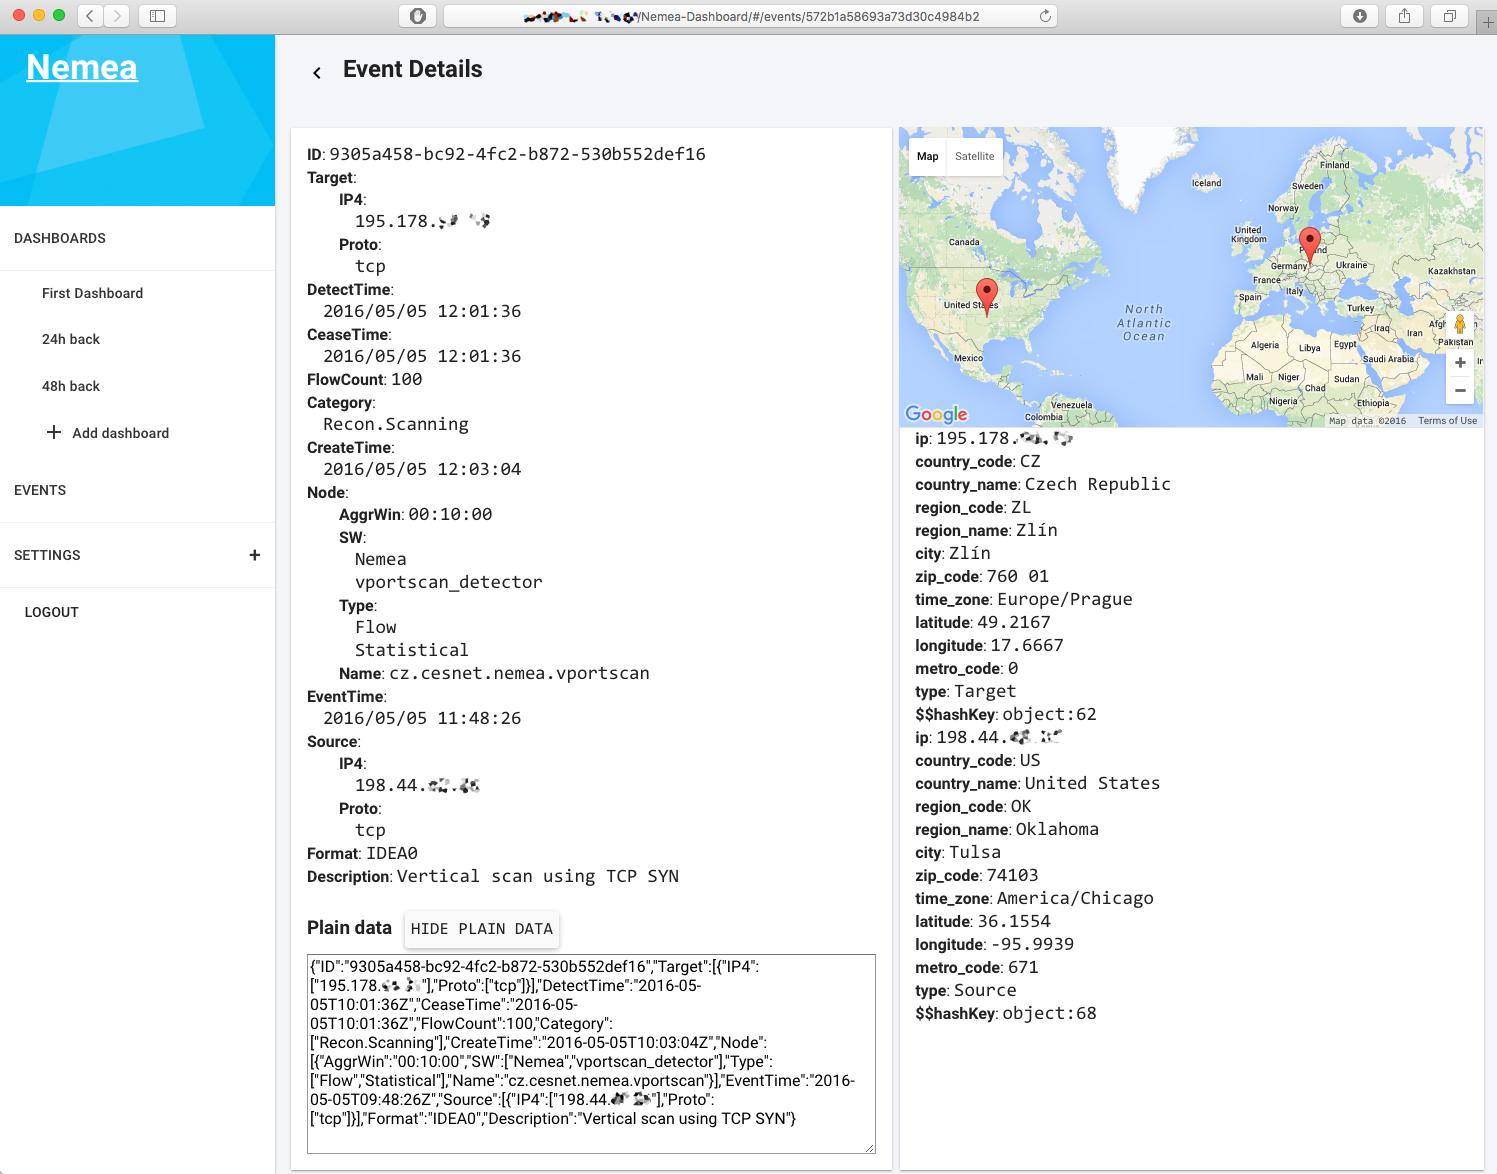
\includegraphics[width=1\textwidth]{fig/screen_after_3.png}
    \caption{Detail události.} \label{screen:after:3}
\end{figure}



\chapter{Obsah DVD}

Na DVD se v kořenovém adresáři nachází následující soubory a složky:

\begin{description}
    \item \texttt{README.txt} popis obsahu DVD.
    \item \texttt{src/} adresář se zdrojovými soubory vytvořené aplikace NEMEA Dashboard.
    \item \texttt{doc/} adresář se zdrojovými kódy této práce.
    \item \texttt{disk/} adresář s~obrazem virtuálního počítače s~předinstalovaným systémem NEMEA a~aplikací NEMEA Dashboard včetně demonstračních anonymizovaných událostí v~databázi MongoDB.
\end{description}
